\documentclass[twoside]{book}

% Packages required by doxygen
\usepackage{calc}
\usepackage{doxygen}
\usepackage{graphicx}
\usepackage[utf8]{inputenc}
\usepackage{makeidx}
\usepackage{multicol}
\usepackage{multirow}
\usepackage{textcomp}
\usepackage[table]{xcolor}

% Font selection
\usepackage[T1]{fontenc}
\usepackage{mathptmx}
\usepackage[scaled=.90]{helvet}
\usepackage{courier}
\usepackage{amssymb}
\usepackage{sectsty}
\renewcommand{\familydefault}{\sfdefault}
\allsectionsfont{%
  \fontseries{bc}\selectfont%
  \color{darkgray}%
}
\renewcommand{\DoxyLabelFont}{%
  \fontseries{bc}\selectfont%
  \color{darkgray}%
}

% Page & text layout
\usepackage{geometry}
\geometry{%
  a4paper,%
  top=2.5cm,%
  bottom=2.5cm,%
  left=2.5cm,%
  right=2.5cm%
}
\tolerance=750
\hfuzz=15pt
\hbadness=750
\setlength{\emergencystretch}{15pt}
\setlength{\parindent}{0cm}
\setlength{\parskip}{0.2cm}
\makeatletter
\renewcommand{\paragraph}{%
  \@startsection{paragraph}{4}{0ex}{-1.0ex}{1.0ex}{%
    \normalfont\normalsize\bfseries\SS@parafont%
  }%
}
\renewcommand{\subparagraph}{%
  \@startsection{subparagraph}{5}{0ex}{-1.0ex}{1.0ex}{%
    \normalfont\normalsize\bfseries\SS@subparafont%
  }%
}
\makeatother

% Headers & footers
\usepackage{fancyhdr}
\pagestyle{fancyplain}
\fancyhead[LE]{\fancyplain{}{\bfseries\thepage}}
\fancyhead[CE]{\fancyplain{}{}}
\fancyhead[RE]{\fancyplain{}{\bfseries\leftmark}}
\fancyhead[LO]{\fancyplain{}{\bfseries\rightmark}}
\fancyhead[CO]{\fancyplain{}{}}
\fancyhead[RO]{\fancyplain{}{\bfseries\thepage}}
\fancyfoot[LE]{\fancyplain{}{}}
\fancyfoot[CE]{\fancyplain{}{}}
\fancyfoot[RE]{\fancyplain{}{\bfseries\scriptsize Generated on Tue Sep 24 2013 09\-:16\-:21 for Python Olog Client Library by Doxygen }}
\fancyfoot[LO]{\fancyplain{}{\bfseries\scriptsize Generated on Tue Sep 24 2013 09\-:16\-:21 for Python Olog Client Library by Doxygen }}
\fancyfoot[CO]{\fancyplain{}{}}
\fancyfoot[RO]{\fancyplain{}{}}
\renewcommand{\footrulewidth}{0.4pt}
\renewcommand{\chaptermark}[1]{%
  \markboth{#1}{}%
}
\renewcommand{\sectionmark}[1]{%
  \markright{\thesection\ #1}%
}

% Indices & bibliography
\usepackage{natbib}
\usepackage[titles]{tocloft}
\setcounter{tocdepth}{3}
\setcounter{secnumdepth}{5}
\makeindex

% Hyperlinks (required, but should be loaded last)
\usepackage{ifpdf}
\ifpdf
  \usepackage[pdftex,pagebackref=true]{hyperref}
\else
  \usepackage[ps2pdf,pagebackref=true]{hyperref}
\fi
\hypersetup{%
  colorlinks=true,%
  linkcolor=blue,%
  citecolor=blue,%
  unicode%
}

% Custom commands
\newcommand{\clearemptydoublepage}{%
  \newpage{\pagestyle{empty}\cleardoublepage}%
}


%===== C O N T E N T S =====

\begin{document}

% Titlepage & ToC
\hypersetup{pageanchor=false}
\pagenumbering{roman}
\begin{titlepage}
\vspace*{7cm}
\begin{center}%
{\Large Python Olog Client Library \\[1ex]\large 2.\-2.\-4-\/\-S\-N\-A\-P\-S\-H\-O\-T }\\
\vspace*{1cm}
{\large Generated by Doxygen 1.8.5}\\
\vspace*{0.5cm}
{\small Tue Sep 24 2013 09:16:21}\\
\end{center}
\end{titlepage}
\clearemptydoublepage
\tableofcontents
\clearemptydoublepage
\pagenumbering{arabic}
\hypersetup{pageanchor=true}

%--- Begin generated contents ---
\chapter{Namespace Index}
\section{Namespace List}
Here is a list of all documented namespaces with brief descriptions\-:\begin{DoxyCompactList}
\item\contentsline{section}{\hyperlink{namespacepyOlog_1_1OlogClient}{py\-Olog.\-Olog\-Client} }{\pageref{namespacepyOlog_1_1OlogClient}}{}
\item\contentsline{section}{\hyperlink{namespacepyOlog_1_1OlogDataTypes}{py\-Olog.\-Olog\-Data\-Types} }{\pageref{namespacepyOlog_1_1OlogDataTypes}}{}
\end{DoxyCompactList}

\chapter{Hierarchical Index}
\section{Class Hierarchy}
This inheritance list is sorted roughly, but not completely, alphabetically\-:\begin{DoxyCompactList}
\item object\begin{DoxyCompactList}
\item \contentsline{section}{py\-Olog.\-Olog\-Client.\-Olog\-Client}{\pageref{classpyOlog_1_1OlogClient_1_1OlogClient}}{}
\item \contentsline{section}{py\-Olog.\-Olog\-Data\-Types.\-Attachment}{\pageref{classpyOlog_1_1OlogDataTypes_1_1Attachment}}{}
\item \contentsline{section}{py\-Olog.\-Olog\-Data\-Types.\-Logbook}{\pageref{classpyOlog_1_1OlogDataTypes_1_1Logbook}}{}
\item \contentsline{section}{py\-Olog.\-Olog\-Data\-Types.\-Log\-Entry}{\pageref{classpyOlog_1_1OlogDataTypes_1_1LogEntry}}{}
\item \contentsline{section}{py\-Olog.\-Olog\-Data\-Types.\-Property}{\pageref{classpyOlog_1_1OlogDataTypes_1_1Property}}{}
\item \contentsline{section}{py\-Olog.\-Olog\-Data\-Types.\-Tag}{\pageref{classpyOlog_1_1OlogDataTypes_1_1Tag}}{}
\end{DoxyCompactList}
\item J\-S\-O\-N\-Decoder\begin{DoxyCompactList}
\item \contentsline{section}{py\-Olog.\-Olog\-Client.\-Logbook\-Decoder}{\pageref{classpyOlog_1_1OlogClient_1_1LogbookDecoder}}{}
\item \contentsline{section}{py\-Olog.\-Olog\-Client.\-Log\-Entry\-Decoder}{\pageref{classpyOlog_1_1OlogClient_1_1LogEntryDecoder}}{}
\item \contentsline{section}{py\-Olog.\-Olog\-Client.\-Property\-Decoder}{\pageref{classpyOlog_1_1OlogClient_1_1PropertyDecoder}}{}
\item \contentsline{section}{py\-Olog.\-Olog\-Client.\-Tag\-Decoder}{\pageref{classpyOlog_1_1OlogClient_1_1TagDecoder}}{}
\end{DoxyCompactList}
\item J\-S\-O\-N\-Encoder\begin{DoxyCompactList}
\item \contentsline{section}{py\-Olog.\-Olog\-Client.\-Logbook\-Encoder}{\pageref{classpyOlog_1_1OlogClient_1_1LogbookEncoder}}{}
\item \contentsline{section}{py\-Olog.\-Olog\-Client.\-Log\-Entry\-Encoder}{\pageref{classpyOlog_1_1OlogClient_1_1LogEntryEncoder}}{}
\item \contentsline{section}{py\-Olog.\-Olog\-Client.\-Property\-Encoder}{\pageref{classpyOlog_1_1OlogClient_1_1PropertyEncoder}}{}
\item \contentsline{section}{py\-Olog.\-Olog\-Client.\-Tag\-Encoder}{\pageref{classpyOlog_1_1OlogClient_1_1TagEncoder}}{}
\end{DoxyCompactList}
\end{DoxyCompactList}

\chapter{Class Index}
\section{Class List}
Here are the classes, structs, unions and interfaces with brief descriptions\-:\begin{DoxyCompactList}
\item\contentsline{section}{\hyperlink{classpyOlog_1_1OlogDataTypes_1_1Attachment}{py\-Olog.\-Olog\-Data\-Types.\-Attachment} }{\pageref{classpyOlog_1_1OlogDataTypes_1_1Attachment}}{}
\item\contentsline{section}{\hyperlink{classpyOlog_1_1OlogDataTypes_1_1Logbook}{py\-Olog.\-Olog\-Data\-Types.\-Logbook} }{\pageref{classpyOlog_1_1OlogDataTypes_1_1Logbook}}{}
\item\contentsline{section}{\hyperlink{classpyOlog_1_1OlogClient_1_1LogbookDecoder}{py\-Olog.\-Olog\-Client.\-Logbook\-Decoder} }{\pageref{classpyOlog_1_1OlogClient_1_1LogbookDecoder}}{}
\item\contentsline{section}{\hyperlink{classpyOlog_1_1OlogClient_1_1LogbookEncoder}{py\-Olog.\-Olog\-Client.\-Logbook\-Encoder} }{\pageref{classpyOlog_1_1OlogClient_1_1LogbookEncoder}}{}
\item\contentsline{section}{\hyperlink{classpyOlog_1_1OlogDataTypes_1_1LogEntry}{py\-Olog.\-Olog\-Data\-Types.\-Log\-Entry} }{\pageref{classpyOlog_1_1OlogDataTypes_1_1LogEntry}}{}
\item\contentsline{section}{\hyperlink{classpyOlog_1_1OlogClient_1_1LogEntryDecoder}{py\-Olog.\-Olog\-Client.\-Log\-Entry\-Decoder} }{\pageref{classpyOlog_1_1OlogClient_1_1LogEntryDecoder}}{}
\item\contentsline{section}{\hyperlink{classpyOlog_1_1OlogClient_1_1LogEntryEncoder}{py\-Olog.\-Olog\-Client.\-Log\-Entry\-Encoder} }{\pageref{classpyOlog_1_1OlogClient_1_1LogEntryEncoder}}{}
\item\contentsline{section}{\hyperlink{classpyOlog_1_1OlogClient_1_1OlogClient}{py\-Olog.\-Olog\-Client.\-Olog\-Client} }{\pageref{classpyOlog_1_1OlogClient_1_1OlogClient}}{}
\item\contentsline{section}{\hyperlink{classpyOlog_1_1OlogDataTypes_1_1Property}{py\-Olog.\-Olog\-Data\-Types.\-Property} }{\pageref{classpyOlog_1_1OlogDataTypes_1_1Property}}{}
\item\contentsline{section}{\hyperlink{classpyOlog_1_1OlogClient_1_1PropertyDecoder}{py\-Olog.\-Olog\-Client.\-Property\-Decoder} }{\pageref{classpyOlog_1_1OlogClient_1_1PropertyDecoder}}{}
\item\contentsline{section}{\hyperlink{classpyOlog_1_1OlogClient_1_1PropertyEncoder}{py\-Olog.\-Olog\-Client.\-Property\-Encoder} }{\pageref{classpyOlog_1_1OlogClient_1_1PropertyEncoder}}{}
\item\contentsline{section}{\hyperlink{classpyOlog_1_1OlogDataTypes_1_1Tag}{py\-Olog.\-Olog\-Data\-Types.\-Tag} }{\pageref{classpyOlog_1_1OlogDataTypes_1_1Tag}}{}
\item\contentsline{section}{\hyperlink{classpyOlog_1_1OlogClient_1_1TagDecoder}{py\-Olog.\-Olog\-Client.\-Tag\-Decoder} }{\pageref{classpyOlog_1_1OlogClient_1_1TagDecoder}}{}
\item\contentsline{section}{\hyperlink{classpyOlog_1_1OlogClient_1_1TagEncoder}{py\-Olog.\-Olog\-Client.\-Tag\-Encoder} }{\pageref{classpyOlog_1_1OlogClient_1_1TagEncoder}}{}
\end{DoxyCompactList}

\chapter{Namespace Documentation}
\hypertarget{namespacepyOlog_1_1OlogClient}{\section{py\-Olog.\-Olog\-Client Namespace Reference}
\label{namespacepyOlog_1_1OlogClient}\index{py\-Olog.\-Olog\-Client@{py\-Olog.\-Olog\-Client}}
}
\subsection*{Classes}
\begin{DoxyCompactItemize}
\item 
class \hyperlink{classpyOlog_1_1OlogClient_1_1OlogClient}{Olog\-Client}
\item 
class \hyperlink{classpyOlog_1_1OlogClient_1_1PropertyEncoder}{Property\-Encoder}
\item 
class \hyperlink{classpyOlog_1_1OlogClient_1_1PropertyDecoder}{Property\-Decoder}
\item 
class \hyperlink{classpyOlog_1_1OlogClient_1_1LogbookEncoder}{Logbook\-Encoder}
\item 
class \hyperlink{classpyOlog_1_1OlogClient_1_1LogbookDecoder}{Logbook\-Decoder}
\item 
class \hyperlink{classpyOlog_1_1OlogClient_1_1TagEncoder}{Tag\-Encoder}
\item 
class \hyperlink{classpyOlog_1_1OlogClient_1_1TagDecoder}{Tag\-Decoder}
\item 
class \hyperlink{classpyOlog_1_1OlogClient_1_1LogEntryEncoder}{Log\-Entry\-Encoder}
\item 
class \hyperlink{classpyOlog_1_1OlogClient_1_1LogEntryDecoder}{Log\-Entry\-Decoder}
\end{DoxyCompactItemize}


\subsection{Detailed Description}
\begin{DoxyVerb}Copyright (c) 2010 Brookhaven National Laboratory
All rights reserved. Use is subject to license terms and conditions.

Created on Jan 10, 2013

@author: shroffk
\end{DoxyVerb}
 
\hypertarget{namespacepyOlog_1_1OlogDataTypes}{\section{py\-Olog.\-Olog\-Data\-Types Namespace Reference}
\label{namespacepyOlog_1_1OlogDataTypes}\index{py\-Olog.\-Olog\-Data\-Types@{py\-Olog.\-Olog\-Data\-Types}}
}
\subsection*{Classes}
\begin{DoxyCompactItemize}
\item 
class \hyperlink{classpyOlog_1_1OlogDataTypes_1_1LogEntry}{Log\-Entry}
\item 
class \hyperlink{classpyOlog_1_1OlogDataTypes_1_1Logbook}{Logbook}
\item 
class \hyperlink{classpyOlog_1_1OlogDataTypes_1_1Tag}{Tag}
\item 
class \hyperlink{classpyOlog_1_1OlogDataTypes_1_1Attachment}{Attachment}
\item 
class \hyperlink{classpyOlog_1_1OlogDataTypes_1_1Property}{Property}
\end{DoxyCompactItemize}


\subsection{Detailed Description}
\begin{DoxyVerb}Copyright (c) 2010 Brookhaven National Laboratory
All rights reserved. Use is subject to license terms and conditions.

Created on Jan 10, 2013

@author: shroffk
\end{DoxyVerb}
 
\chapter{Class Documentation}
\hypertarget{classpyOlog_1_1OlogDataTypes_1_1Attachment}{\section{py\-Olog.\-Olog\-Data\-Types.\-Attachment Class Reference}
\label{classpyOlog_1_1OlogDataTypes_1_1Attachment}\index{py\-Olog.\-Olog\-Data\-Types.\-Attachment@{py\-Olog.\-Olog\-Data\-Types.\-Attachment}}
}
Inheritance diagram for py\-Olog.\-Olog\-Data\-Types.\-Attachment\-:\begin{figure}[H]
\begin{center}
\leavevmode
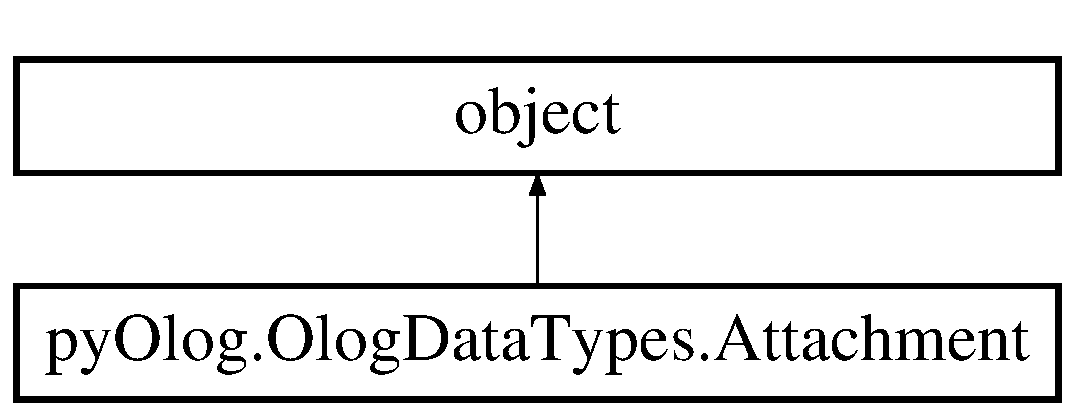
\includegraphics[height=2.000000cm]{classpyOlog_1_1OlogDataTypes_1_1Attachment}
\end{center}
\end{figure}
\subsection*{Public Member Functions}
\begin{DoxyCompactItemize}
\item 
def \hyperlink{classpyOlog_1_1OlogDataTypes_1_1Attachment_adee39c9ec988dcc8edc84109fb8ffa9d}{\-\_\-\-\_\-init\-\_\-\-\_\-}
\item 
\hypertarget{classpyOlog_1_1OlogDataTypes_1_1Attachment_a08d8430ba6e93b4ca662ff13f13d0fae}{def {\bfseries get\-File}}\label{classpyOlog_1_1OlogDataTypes_1_1Attachment_a08d8430ba6e93b4ca662ff13f13d0fae}

\end{DoxyCompactItemize}


\subsection{Detailed Description}
\begin{DoxyVerb}A Attachment, a file associated with the log entry
TODO this is not thread safe    
\end{DoxyVerb}
 

\subsection{Constructor \& Destructor Documentation}
\hypertarget{classpyOlog_1_1OlogDataTypes_1_1Attachment_adee39c9ec988dcc8edc84109fb8ffa9d}{\index{py\-Olog\-::\-Olog\-Data\-Types\-::\-Attachment@{py\-Olog\-::\-Olog\-Data\-Types\-::\-Attachment}!\-\_\-\-\_\-init\-\_\-\-\_\-@{\-\_\-\-\_\-init\-\_\-\-\_\-}}
\index{\-\_\-\-\_\-init\-\_\-\-\_\-@{\-\_\-\-\_\-init\-\_\-\-\_\-}!pyOlog::OlogDataTypes::Attachment@{py\-Olog\-::\-Olog\-Data\-Types\-::\-Attachment}}
\subsubsection[{\-\_\-\-\_\-init\-\_\-\-\_\-}]{\setlength{\rightskip}{0pt plus 5cm}def py\-Olog.\-Olog\-Data\-Types.\-Attachment.\-\_\-\-\_\-init\-\_\-\-\_\- (
\begin{DoxyParamCaption}
\item[{}]{self, }
\item[{}]{file}
\end{DoxyParamCaption}
)}}\label{classpyOlog_1_1OlogDataTypes_1_1Attachment_adee39c9ec988dcc8edc84109fb8ffa9d}
\begin{DoxyVerb}Create Attachment 
>> Attachment(file=open('/home/usr/databrowser.plt')
>> Attachment(file=open('test.jpg','rb')
\end{DoxyVerb}
 

The documentation for this class was generated from the following file\-:\begin{DoxyCompactItemize}
\item 
py\-Olog/Olog\-Data\-Types.\-py\end{DoxyCompactItemize}

\hypertarget{classpyOlog_1_1OlogDataTypes_1_1Logbook}{\section{py\-Olog.\-Olog\-Data\-Types.\-Logbook Class Reference}
\label{classpyOlog_1_1OlogDataTypes_1_1Logbook}\index{py\-Olog.\-Olog\-Data\-Types.\-Logbook@{py\-Olog.\-Olog\-Data\-Types.\-Logbook}}
}
Inheritance diagram for py\-Olog.\-Olog\-Data\-Types.\-Logbook\-:\begin{figure}[H]
\begin{center}
\leavevmode
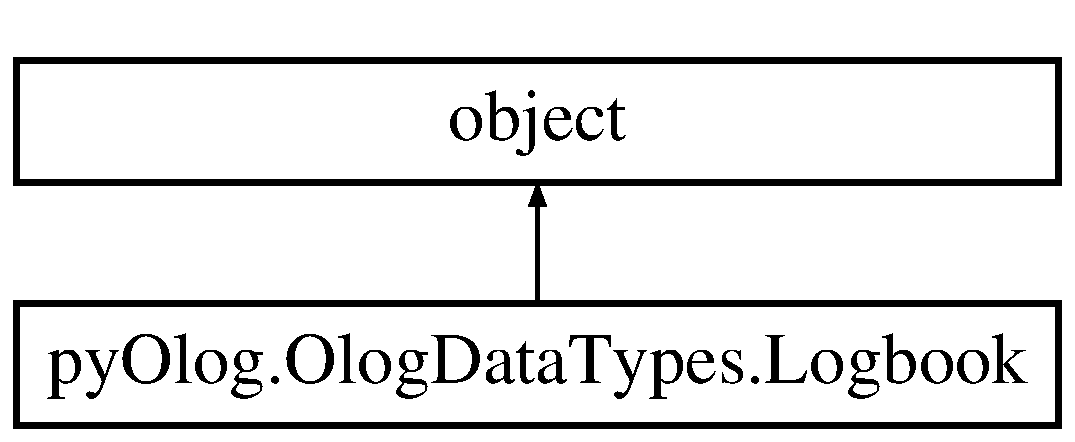
\includegraphics[height=2.000000cm]{classpyOlog_1_1OlogDataTypes_1_1Logbook}
\end{center}
\end{figure}
\subsection*{Public Member Functions}
\begin{DoxyCompactItemize}
\item 
def \hyperlink{classpyOlog_1_1OlogDataTypes_1_1Logbook_a98e02bb45dcbfeecc9e943e80e5ba0f8}{\-\_\-\-\_\-init\-\_\-\-\_\-}
\item 
\hypertarget{classpyOlog_1_1OlogDataTypes_1_1Logbook_ae39aeb8825d2138c1ff43d7c50366795}{def {\bfseries get\-Name}}\label{classpyOlog_1_1OlogDataTypes_1_1Logbook_ae39aeb8825d2138c1ff43d7c50366795}

\item 
\hypertarget{classpyOlog_1_1OlogDataTypes_1_1Logbook_a98510d4f009cf86a29003df5905c8727}{def {\bfseries get\-Owner}}\label{classpyOlog_1_1OlogDataTypes_1_1Logbook_a98510d4f009cf86a29003df5905c8727}

\item 
\hypertarget{classpyOlog_1_1OlogDataTypes_1_1Logbook_a7fcc126baf6e6921b512228e0217e438}{def {\bfseries \-\_\-\-\_\-cmp\-\_\-\-\_\-}}\label{classpyOlog_1_1OlogDataTypes_1_1Logbook_a7fcc126baf6e6921b512228e0217e438}

\end{DoxyCompactItemize}


\subsection{Detailed Description}
\begin{DoxyVerb}A Logbook consist of an unique name and an owner, 
logentries can be added to a logbook so long as the user either the owner
or a member of the owner group
\end{DoxyVerb}
 

\subsection{Constructor \& Destructor Documentation}
\hypertarget{classpyOlog_1_1OlogDataTypes_1_1Logbook_a98e02bb45dcbfeecc9e943e80e5ba0f8}{\index{py\-Olog\-::\-Olog\-Data\-Types\-::\-Logbook@{py\-Olog\-::\-Olog\-Data\-Types\-::\-Logbook}!\-\_\-\-\_\-init\-\_\-\-\_\-@{\-\_\-\-\_\-init\-\_\-\-\_\-}}
\index{\-\_\-\-\_\-init\-\_\-\-\_\-@{\-\_\-\-\_\-init\-\_\-\-\_\-}!pyOlog::OlogDataTypes::Logbook@{py\-Olog\-::\-Olog\-Data\-Types\-::\-Logbook}}
\subsubsection[{\-\_\-\-\_\-init\-\_\-\-\_\-}]{\setlength{\rightskip}{0pt plus 5cm}def py\-Olog.\-Olog\-Data\-Types.\-Logbook.\-\_\-\-\_\-init\-\_\-\-\_\- (
\begin{DoxyParamCaption}
\item[{}]{self, }
\item[{}]{name, }
\item[{}]{owner}
\end{DoxyParamCaption}
)}}\label{classpyOlog_1_1OlogDataTypes_1_1Logbook_a98e02bb45dcbfeecc9e943e80e5ba0f8}
\begin{DoxyVerb}Create a logbook
>> Logbook('commissioning', 'controls')
\end{DoxyVerb}
 

The documentation for this class was generated from the following file\-:\begin{DoxyCompactItemize}
\item 
py\-Olog/Olog\-Data\-Types.\-py\end{DoxyCompactItemize}

\hypertarget{classpyOlog_1_1OlogClient_1_1LogbookDecoder}{\section{py\-Olog.\-Olog\-Client.\-Logbook\-Decoder Class Reference}
\label{classpyOlog_1_1OlogClient_1_1LogbookDecoder}\index{py\-Olog.\-Olog\-Client.\-Logbook\-Decoder@{py\-Olog.\-Olog\-Client.\-Logbook\-Decoder}}
}
Inheritance diagram for py\-Olog.\-Olog\-Client.\-Logbook\-Decoder\-:\begin{figure}[H]
\begin{center}
\leavevmode
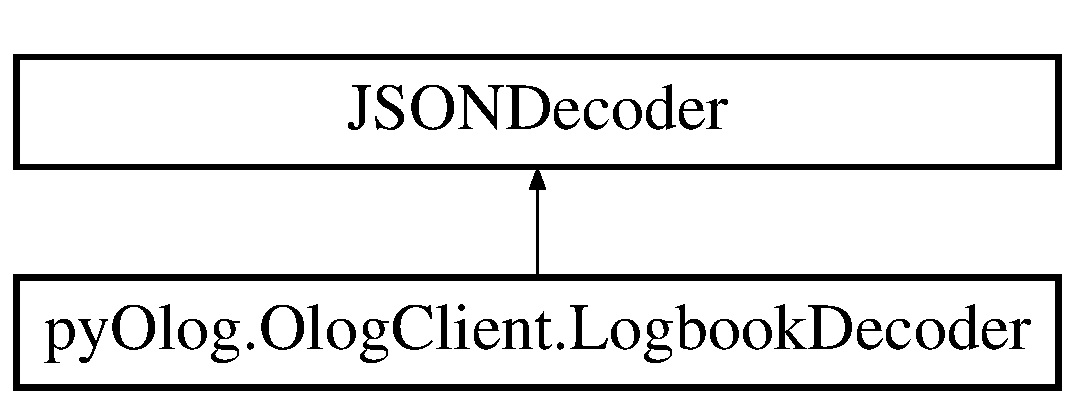
\includegraphics[height=2.000000cm]{classpyOlog_1_1OlogClient_1_1LogbookDecoder}
\end{center}
\end{figure}
\subsection*{Public Member Functions}
\begin{DoxyCompactItemize}
\item 
\hypertarget{classpyOlog_1_1OlogClient_1_1LogbookDecoder_ae58c55891533f4eaa7cab68f454c71ee}{def {\bfseries \-\_\-\-\_\-init\-\_\-\-\_\-}}\label{classpyOlog_1_1OlogClient_1_1LogbookDecoder_ae58c55891533f4eaa7cab68f454c71ee}

\item 
\hypertarget{classpyOlog_1_1OlogClient_1_1LogbookDecoder_ad56ae6f4fd18c4d21a311c37b0e817ef}{def {\bfseries dict\-To\-Logbook}}\label{classpyOlog_1_1OlogClient_1_1LogbookDecoder_ad56ae6f4fd18c4d21a311c37b0e817ef}

\end{DoxyCompactItemize}


The documentation for this class was generated from the following file\-:\begin{DoxyCompactItemize}
\item 
py\-Olog/Olog\-Client.\-py\end{DoxyCompactItemize}

\hypertarget{classpyOlog_1_1OlogClient_1_1LogbookEncoder}{\section{py\-Olog.\-Olog\-Client.\-Logbook\-Encoder Class Reference}
\label{classpyOlog_1_1OlogClient_1_1LogbookEncoder}\index{py\-Olog.\-Olog\-Client.\-Logbook\-Encoder@{py\-Olog.\-Olog\-Client.\-Logbook\-Encoder}}
}
Inheritance diagram for py\-Olog.\-Olog\-Client.\-Logbook\-Encoder\-:\begin{figure}[H]
\begin{center}
\leavevmode
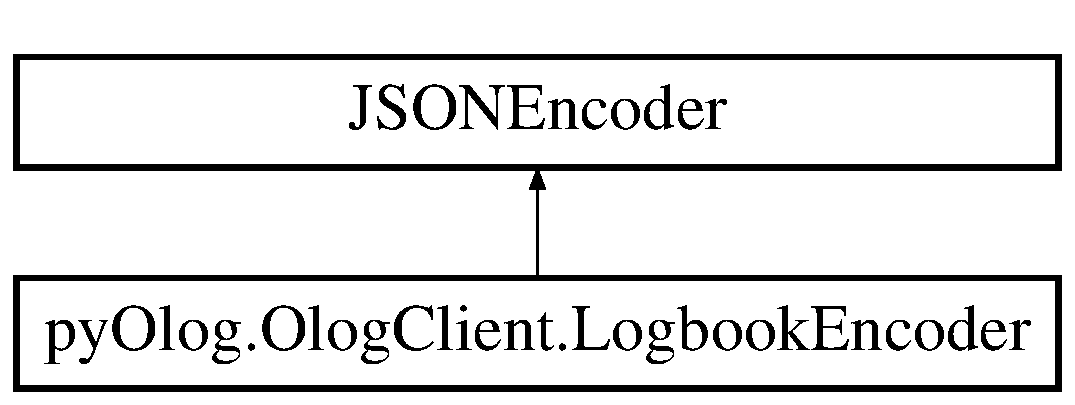
\includegraphics[height=2.000000cm]{classpyOlog_1_1OlogClient_1_1LogbookEncoder}
\end{center}
\end{figure}
\subsection*{Public Member Functions}
\begin{DoxyCompactItemize}
\item 
\hypertarget{classpyOlog_1_1OlogClient_1_1LogbookEncoder_a8c72391004f85cbd0f749b0171ce0baa}{def {\bfseries default}}\label{classpyOlog_1_1OlogClient_1_1LogbookEncoder_a8c72391004f85cbd0f749b0171ce0baa}

\end{DoxyCompactItemize}


The documentation for this class was generated from the following file\-:\begin{DoxyCompactItemize}
\item 
py\-Olog/Olog\-Client.\-py\end{DoxyCompactItemize}

\hypertarget{classpyOlog_1_1OlogDataTypes_1_1LogEntry}{\section{py\-Olog.\-Olog\-Data\-Types.\-Log\-Entry Class Reference}
\label{classpyOlog_1_1OlogDataTypes_1_1LogEntry}\index{py\-Olog.\-Olog\-Data\-Types.\-Log\-Entry@{py\-Olog.\-Olog\-Data\-Types.\-Log\-Entry}}
}
Inheritance diagram for py\-Olog.\-Olog\-Data\-Types.\-Log\-Entry\-:\begin{figure}[H]
\begin{center}
\leavevmode
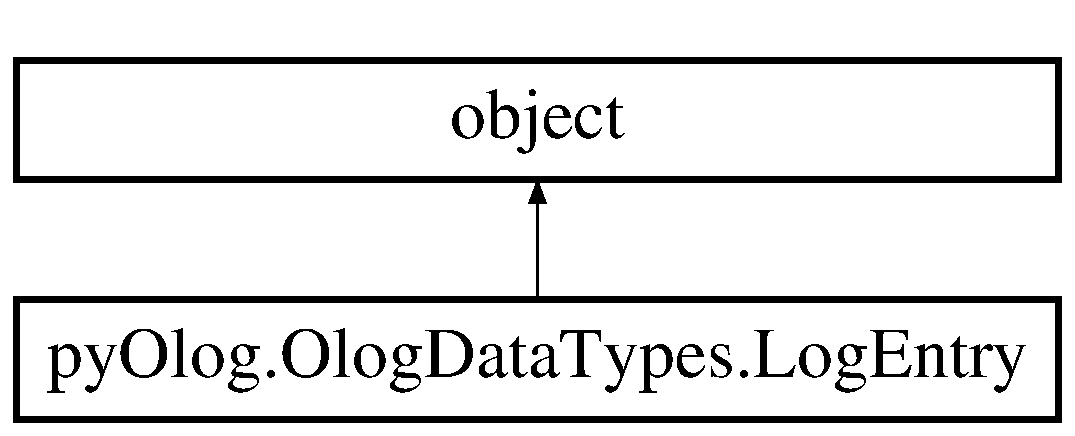
\includegraphics[height=2.000000cm]{classpyOlog_1_1OlogDataTypes_1_1LogEntry}
\end{center}
\end{figure}
\subsection*{Public Member Functions}
\begin{DoxyCompactItemize}
\item 
def \hyperlink{classpyOlog_1_1OlogDataTypes_1_1LogEntry_a13bf1f416e5bee9a944926e33b427fcd}{\-\_\-\-\_\-init\-\_\-\-\_\-}
\item 
\hypertarget{classpyOlog_1_1OlogDataTypes_1_1LogEntry_a672284e5f0662d1858aa5881ef47f8be}{def {\bfseries get\-Id}}\label{classpyOlog_1_1OlogDataTypes_1_1LogEntry_a672284e5f0662d1858aa5881ef47f8be}

\item 
\hypertarget{classpyOlog_1_1OlogDataTypes_1_1LogEntry_a59f60a7850fa72b5a70766573da665df}{def {\bfseries get\-Create\-Time}}\label{classpyOlog_1_1OlogDataTypes_1_1LogEntry_a59f60a7850fa72b5a70766573da665df}

\item 
\hypertarget{classpyOlog_1_1OlogDataTypes_1_1LogEntry_ac93331a643dec6d524ef8f39d5b57444}{def {\bfseries get\-Modify\-Time}}\label{classpyOlog_1_1OlogDataTypes_1_1LogEntry_ac93331a643dec6d524ef8f39d5b57444}

\item 
\hypertarget{classpyOlog_1_1OlogDataTypes_1_1LogEntry_a92d03e0011c826876e520fc8807a5b97}{def {\bfseries get\-Text}}\label{classpyOlog_1_1OlogDataTypes_1_1LogEntry_a92d03e0011c826876e520fc8807a5b97}

\item 
\hypertarget{classpyOlog_1_1OlogDataTypes_1_1LogEntry_a8a1353f4981b3cb1c448259d87a8be70}{def {\bfseries get\-Owner}}\label{classpyOlog_1_1OlogDataTypes_1_1LogEntry_a8a1353f4981b3cb1c448259d87a8be70}

\item 
\hypertarget{classpyOlog_1_1OlogDataTypes_1_1LogEntry_a936a44ddc8fae71244990b721798d833}{def {\bfseries get\-Logbooks}}\label{classpyOlog_1_1OlogDataTypes_1_1LogEntry_a936a44ddc8fae71244990b721798d833}

\item 
\hypertarget{classpyOlog_1_1OlogDataTypes_1_1LogEntry_a94d1b849d15282ccbb65650b0726440f}{def {\bfseries get\-Tags}}\label{classpyOlog_1_1OlogDataTypes_1_1LogEntry_a94d1b849d15282ccbb65650b0726440f}

\item 
\hypertarget{classpyOlog_1_1OlogDataTypes_1_1LogEntry_a9ec5d7b29198de3e784c9e4c8505483d}{def {\bfseries get\-Attachments}}\label{classpyOlog_1_1OlogDataTypes_1_1LogEntry_a9ec5d7b29198de3e784c9e4c8505483d}

\item 
\hypertarget{classpyOlog_1_1OlogDataTypes_1_1LogEntry_a38dbad758bb5169e91ecdd70642ee174}{def {\bfseries get\-Properties}}\label{classpyOlog_1_1OlogDataTypes_1_1LogEntry_a38dbad758bb5169e91ecdd70642ee174}

\item 
\hypertarget{classpyOlog_1_1OlogDataTypes_1_1LogEntry_a5ed9da188a34dda8da858c4064c8edd9}{def {\bfseries \-\_\-\-\_\-cmp\-\_\-\-\_\-}}\label{classpyOlog_1_1OlogDataTypes_1_1LogEntry_a5ed9da188a34dda8da858c4064c8edd9}

\end{DoxyCompactItemize}
\subsection*{Public Attributes}
\begin{DoxyCompactItemize}
\item 
\hypertarget{classpyOlog_1_1OlogDataTypes_1_1LogEntry_a40d5d1b940636347305c7da17c6e06b0}{{\bfseries Text}}\label{classpyOlog_1_1OlogDataTypes_1_1LogEntry_a40d5d1b940636347305c7da17c6e06b0}

\item 
\hypertarget{classpyOlog_1_1OlogDataTypes_1_1LogEntry_afe85d9e93b0abfc9f7c895a9f83f7589}{{\bfseries Owner}}\label{classpyOlog_1_1OlogDataTypes_1_1LogEntry_afe85d9e93b0abfc9f7c895a9f83f7589}

\item 
\hypertarget{classpyOlog_1_1OlogDataTypes_1_1LogEntry_a4f36500a6a6e2575c53bc4d5cfec392c}{{\bfseries logbooks}}\label{classpyOlog_1_1OlogDataTypes_1_1LogEntry_a4f36500a6a6e2575c53bc4d5cfec392c}

\item 
\hypertarget{classpyOlog_1_1OlogDataTypes_1_1LogEntry_a21a53922f015cc14b2ea18f0a260e2ca}{{\bfseries tags}}\label{classpyOlog_1_1OlogDataTypes_1_1LogEntry_a21a53922f015cc14b2ea18f0a260e2ca}

\item 
\hypertarget{classpyOlog_1_1OlogDataTypes_1_1LogEntry_a62fc262c06dfcf8ecf623c58f5bcb4cc}{{\bfseries attachments}}\label{classpyOlog_1_1OlogDataTypes_1_1LogEntry_a62fc262c06dfcf8ecf623c58f5bcb4cc}

\item 
\hypertarget{classpyOlog_1_1OlogDataTypes_1_1LogEntry_aa0d46617e6e711d948a710b530f3b161}{{\bfseries properties}}\label{classpyOlog_1_1OlogDataTypes_1_1LogEntry_aa0d46617e6e711d948a710b530f3b161}

\end{DoxyCompactItemize}


\subsection{Detailed Description}
\begin{DoxyVerb}A LogEntry consists of some Text description, an owner and an associated logbook
It can optionally be associated with one or more logbooks and contain one or more tags, properties and attachments
\end{DoxyVerb}
 

\subsection{Constructor \& Destructor Documentation}
\hypertarget{classpyOlog_1_1OlogDataTypes_1_1LogEntry_a13bf1f416e5bee9a944926e33b427fcd}{\index{py\-Olog\-::\-Olog\-Data\-Types\-::\-Log\-Entry@{py\-Olog\-::\-Olog\-Data\-Types\-::\-Log\-Entry}!\-\_\-\-\_\-init\-\_\-\-\_\-@{\-\_\-\-\_\-init\-\_\-\-\_\-}}
\index{\-\_\-\-\_\-init\-\_\-\-\_\-@{\-\_\-\-\_\-init\-\_\-\-\_\-}!pyOlog::OlogDataTypes::LogEntry@{py\-Olog\-::\-Olog\-Data\-Types\-::\-Log\-Entry}}
\subsubsection[{\-\_\-\-\_\-init\-\_\-\-\_\-}]{\setlength{\rightskip}{0pt plus 5cm}def py\-Olog.\-Olog\-Data\-Types.\-Log\-Entry.\-\_\-\-\_\-init\-\_\-\-\_\- (
\begin{DoxyParamCaption}
\item[{}]{self, }
\item[{}]{text, }
\item[{}]{owner, }
\item[{}]{logbooks, }
\item[{}]{tags = {\ttfamily \mbox{[}\mbox{]}}, }
\item[{}]{attachments = {\ttfamily \mbox{[}\mbox{]}}, }
\item[{}]{properties = {\ttfamily \mbox{[}\mbox{]}}, }
\item[{}]{id = {\ttfamily None}, }
\item[{}]{create\-Time = {\ttfamily None}, }
\item[{}]{modify\-Time = {\ttfamily None}}
\end{DoxyParamCaption}
)}}\label{classpyOlog_1_1OlogDataTypes_1_1LogEntry_a13bf1f416e5bee9a944926e33b427fcd}
\begin{DoxyVerb}Constructor for log Entry
Simple LogEntry
>> LogEntry('test log entry', 'controls', logbooks=[Logbook('commissioning', owner='controls')])

Comprehensive logEntry
>> LogEntry('test log entry', 'controls', 
    logbooks=[Logbook('commissioning', owner='controls')],
    tags=[Tag('TimingSystem')]
    properties=[Property('Ticket', attributes={'Id':'1234','URL':'http://trac.nsls2.bnl.gov/trac/1234'}]
    attachments=[Attachment(open('databrowser.plt'))]
    )
\end{DoxyVerb}
 

The documentation for this class was generated from the following file\-:\begin{DoxyCompactItemize}
\item 
py\-Olog/Olog\-Data\-Types.\-py\end{DoxyCompactItemize}

\hypertarget{classpyOlog_1_1OlogClient_1_1LogEntryDecoder}{\section{py\-Olog.\-Olog\-Client.\-Log\-Entry\-Decoder Class Reference}
\label{classpyOlog_1_1OlogClient_1_1LogEntryDecoder}\index{py\-Olog.\-Olog\-Client.\-Log\-Entry\-Decoder@{py\-Olog.\-Olog\-Client.\-Log\-Entry\-Decoder}}
}
Inheritance diagram for py\-Olog.\-Olog\-Client.\-Log\-Entry\-Decoder\-:\begin{figure}[H]
\begin{center}
\leavevmode
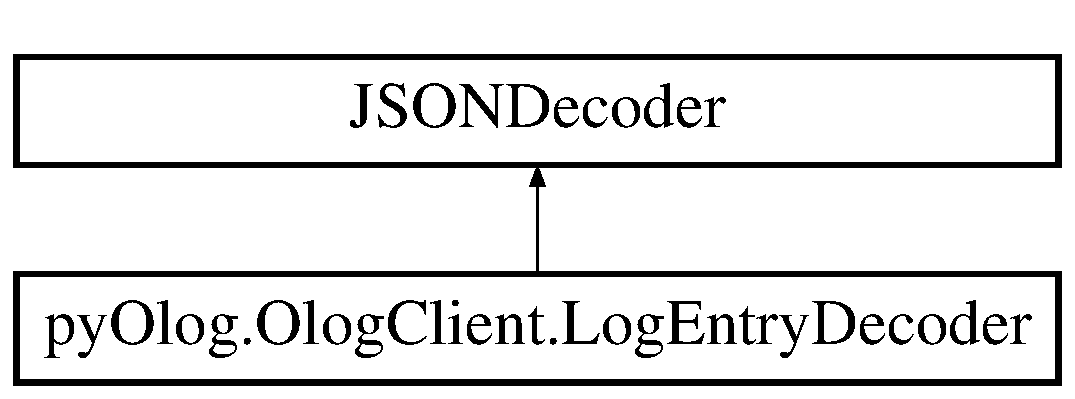
\includegraphics[height=2.000000cm]{classpyOlog_1_1OlogClient_1_1LogEntryDecoder}
\end{center}
\end{figure}
\subsection*{Public Member Functions}
\begin{DoxyCompactItemize}
\item 
\hypertarget{classpyOlog_1_1OlogClient_1_1LogEntryDecoder_a013c24fc1595d6b37ba82cdf93a7b8f7}{def {\bfseries \-\_\-\-\_\-init\-\_\-\-\_\-}}\label{classpyOlog_1_1OlogClient_1_1LogEntryDecoder_a013c24fc1595d6b37ba82cdf93a7b8f7}

\item 
\hypertarget{classpyOlog_1_1OlogClient_1_1LogEntryDecoder_ad910f75e0e8e38d4d09d0e813b6756a1}{def {\bfseries dict\-To\-Log\-Entry}}\label{classpyOlog_1_1OlogClient_1_1LogEntryDecoder_ad910f75e0e8e38d4d09d0e813b6756a1}

\end{DoxyCompactItemize}


The documentation for this class was generated from the following file\-:\begin{DoxyCompactItemize}
\item 
py\-Olog/Olog\-Client.\-py\end{DoxyCompactItemize}

\hypertarget{classpyOlog_1_1OlogClient_1_1LogEntryEncoder}{\section{py\-Olog.\-Olog\-Client.\-Log\-Entry\-Encoder Class Reference}
\label{classpyOlog_1_1OlogClient_1_1LogEntryEncoder}\index{py\-Olog.\-Olog\-Client.\-Log\-Entry\-Encoder@{py\-Olog.\-Olog\-Client.\-Log\-Entry\-Encoder}}
}
Inheritance diagram for py\-Olog.\-Olog\-Client.\-Log\-Entry\-Encoder\-:\begin{figure}[H]
\begin{center}
\leavevmode
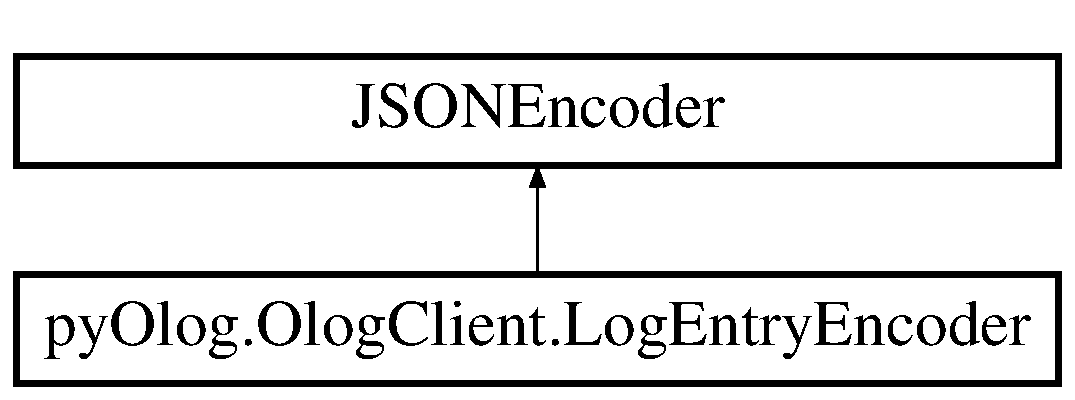
\includegraphics[height=2.000000cm]{classpyOlog_1_1OlogClient_1_1LogEntryEncoder}
\end{center}
\end{figure}
\subsection*{Public Member Functions}
\begin{DoxyCompactItemize}
\item 
\hypertarget{classpyOlog_1_1OlogClient_1_1LogEntryEncoder_a0b7bfb3de48985148b6b53a020b53f98}{def {\bfseries default}}\label{classpyOlog_1_1OlogClient_1_1LogEntryEncoder_a0b7bfb3de48985148b6b53a020b53f98}

\end{DoxyCompactItemize}


The documentation for this class was generated from the following file\-:\begin{DoxyCompactItemize}
\item 
py\-Olog/Olog\-Client.\-py\end{DoxyCompactItemize}

\hypertarget{classpyOlog_1_1OlogClient_1_1OlogClient}{\section{py\-Olog.\-Olog\-Client.\-Olog\-Client Class Reference}
\label{classpyOlog_1_1OlogClient_1_1OlogClient}\index{py\-Olog.\-Olog\-Client.\-Olog\-Client@{py\-Olog.\-Olog\-Client.\-Olog\-Client}}
}
Inheritance diagram for py\-Olog.\-Olog\-Client.\-Olog\-Client\-:\begin{figure}[H]
\begin{center}
\leavevmode
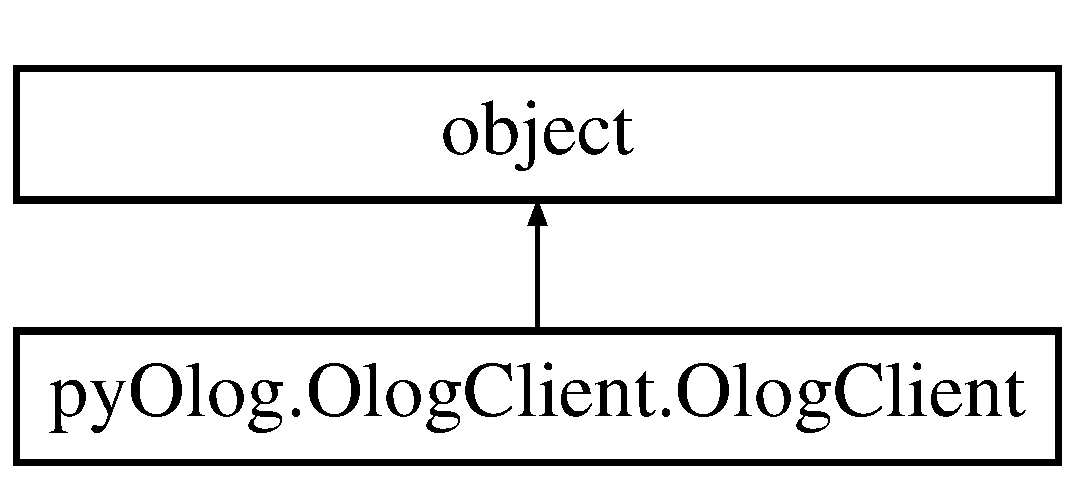
\includegraphics[height=2.000000cm]{classpyOlog_1_1OlogClient_1_1OlogClient}
\end{center}
\end{figure}
\subsection*{Public Member Functions}
\begin{DoxyCompactItemize}
\item 
def \hyperlink{classpyOlog_1_1OlogClient_1_1OlogClient_ae29e50bc4607672b6adeaa73c267030b}{\-\_\-\-\_\-init\-\_\-\-\_\-}
\item 
def \hyperlink{classpyOlog_1_1OlogClient_1_1OlogClient_a8b877d455ef7ebdf879254d8001f53bd}{log}
\item 
def \hyperlink{classpyOlog_1_1OlogClient_1_1OlogClient_aad5b526ddbf6a74259e625d763e503e6}{create\-Logbook}
\item 
def \hyperlink{classpyOlog_1_1OlogClient_1_1OlogClient_a99d70e3e90a5d42ef16c77f6286694d0}{create\-Tag}
\item 
def \hyperlink{classpyOlog_1_1OlogClient_1_1OlogClient_ac4fc7e86a08f87a32f2f3bbbed70b6b7}{create\-Property}
\item 
def \hyperlink{classpyOlog_1_1OlogClient_1_1OlogClient_a29d27bda8fb1172ec677e89246d84353}{find}
\item 
def \hyperlink{classpyOlog_1_1OlogClient_1_1OlogClient_a3d5a89b2130b434d84fb4d8d49e4c701}{list\-Attachments}
\item 
def \hyperlink{classpyOlog_1_1OlogClient_1_1OlogClient_aa0d07acad5b961c3af1fd81be48f33ec}{list\-Tags}
\item 
def \hyperlink{classpyOlog_1_1OlogClient_1_1OlogClient_a6f9af8ff00f272a5150ac1e4c457dfe6}{list\-Logbooks}
\item 
def \hyperlink{classpyOlog_1_1OlogClient_1_1OlogClient_a2609b79d8b10923556b9db7987164239}{list\-Properties}
\item 
def \hyperlink{classpyOlog_1_1OlogClient_1_1OlogClient_a7d072d6a9e63e4a99242d8bdcc20e8db}{delete}
\end{DoxyCompactItemize}


\subsection{Detailed Description}
\begin{DoxyVerb}classdocs
\end{DoxyVerb}
 

\subsection{Constructor \& Destructor Documentation}
\hypertarget{classpyOlog_1_1OlogClient_1_1OlogClient_ae29e50bc4607672b6adeaa73c267030b}{\index{py\-Olog\-::\-Olog\-Client\-::\-Olog\-Client@{py\-Olog\-::\-Olog\-Client\-::\-Olog\-Client}!\-\_\-\-\_\-init\-\_\-\-\_\-@{\-\_\-\-\_\-init\-\_\-\-\_\-}}
\index{\-\_\-\-\_\-init\-\_\-\-\_\-@{\-\_\-\-\_\-init\-\_\-\-\_\-}!pyOlog::OlogClient::OlogClient@{py\-Olog\-::\-Olog\-Client\-::\-Olog\-Client}}
\subsubsection[{\-\_\-\-\_\-init\-\_\-\-\_\-}]{\setlength{\rightskip}{0pt plus 5cm}def py\-Olog.\-Olog\-Client.\-Olog\-Client.\-\_\-\-\_\-init\-\_\-\-\_\- (
\begin{DoxyParamCaption}
\item[{}]{self, }
\item[{}]{url = {\ttfamily None}, }
\item[{}]{username = {\ttfamily None}, }
\item[{}]{password = {\ttfamily None}}
\end{DoxyParamCaption}
)}}\label{classpyOlog_1_1OlogClient_1_1OlogClient_ae29e50bc4607672b6adeaa73c267030b}
\begin{DoxyVerb}Constructor
\end{DoxyVerb}
 

\subsection{Member Function Documentation}
\hypertarget{classpyOlog_1_1OlogClient_1_1OlogClient_aad5b526ddbf6a74259e625d763e503e6}{\index{py\-Olog\-::\-Olog\-Client\-::\-Olog\-Client@{py\-Olog\-::\-Olog\-Client\-::\-Olog\-Client}!create\-Logbook@{create\-Logbook}}
\index{create\-Logbook@{create\-Logbook}!pyOlog::OlogClient::OlogClient@{py\-Olog\-::\-Olog\-Client\-::\-Olog\-Client}}
\subsubsection[{create\-Logbook}]{\setlength{\rightskip}{0pt plus 5cm}def py\-Olog.\-Olog\-Client.\-Olog\-Client.\-create\-Logbook (
\begin{DoxyParamCaption}
\item[{}]{self, }
\item[{}]{logbook}
\end{DoxyParamCaption}
)}}\label{classpyOlog_1_1OlogClient_1_1OlogClient_aad5b526ddbf6a74259e625d763e503e6}
\begin{DoxyVerb}Create Logbook
\end{DoxyVerb}
 \hypertarget{classpyOlog_1_1OlogClient_1_1OlogClient_ac4fc7e86a08f87a32f2f3bbbed70b6b7}{\index{py\-Olog\-::\-Olog\-Client\-::\-Olog\-Client@{py\-Olog\-::\-Olog\-Client\-::\-Olog\-Client}!create\-Property@{create\-Property}}
\index{create\-Property@{create\-Property}!pyOlog::OlogClient::OlogClient@{py\-Olog\-::\-Olog\-Client\-::\-Olog\-Client}}
\subsubsection[{create\-Property}]{\setlength{\rightskip}{0pt plus 5cm}def py\-Olog.\-Olog\-Client.\-Olog\-Client.\-create\-Property (
\begin{DoxyParamCaption}
\item[{}]{self, }
\item[{}]{property}
\end{DoxyParamCaption}
)}}\label{classpyOlog_1_1OlogClient_1_1OlogClient_ac4fc7e86a08f87a32f2f3bbbed70b6b7}
\begin{DoxyVerb}Create Property
\end{DoxyVerb}
 \hypertarget{classpyOlog_1_1OlogClient_1_1OlogClient_a99d70e3e90a5d42ef16c77f6286694d0}{\index{py\-Olog\-::\-Olog\-Client\-::\-Olog\-Client@{py\-Olog\-::\-Olog\-Client\-::\-Olog\-Client}!create\-Tag@{create\-Tag}}
\index{create\-Tag@{create\-Tag}!pyOlog::OlogClient::OlogClient@{py\-Olog\-::\-Olog\-Client\-::\-Olog\-Client}}
\subsubsection[{create\-Tag}]{\setlength{\rightskip}{0pt plus 5cm}def py\-Olog.\-Olog\-Client.\-Olog\-Client.\-create\-Tag (
\begin{DoxyParamCaption}
\item[{}]{self, }
\item[{}]{tag}
\end{DoxyParamCaption}
)}}\label{classpyOlog_1_1OlogClient_1_1OlogClient_a99d70e3e90a5d42ef16c77f6286694d0}
\begin{DoxyVerb}Create Tag
\end{DoxyVerb}
 \hypertarget{classpyOlog_1_1OlogClient_1_1OlogClient_a7d072d6a9e63e4a99242d8bdcc20e8db}{\index{py\-Olog\-::\-Olog\-Client\-::\-Olog\-Client@{py\-Olog\-::\-Olog\-Client\-::\-Olog\-Client}!delete@{delete}}
\index{delete@{delete}!pyOlog::OlogClient::OlogClient@{py\-Olog\-::\-Olog\-Client\-::\-Olog\-Client}}
\subsubsection[{delete}]{\setlength{\rightskip}{0pt plus 5cm}def py\-Olog.\-Olog\-Client.\-Olog\-Client.\-delete (
\begin{DoxyParamCaption}
\item[{}]{self, }
\item[{}]{kwds}
\end{DoxyParamCaption}
)}}\label{classpyOlog_1_1OlogClient_1_1OlogClient_a7d072d6a9e63e4a99242d8bdcc20e8db}
\begin{DoxyVerb}Method to delete a logEntry, logbook, property, tag
delete(logEntryId = int)
>>> delete(logEntryId=1234)

delete(logbookName = String)
>>> delete(logbookName = 'logbookName')

delete(tagName = String)
>>> delete(tagName = 'myTag')
# tagName = tag name of the tag to be deleted (it will be removed from all logEntries)

delete(propertyName = String)
>>> delete(propertyName = 'position')
# propertyName = property name of property to be deleted (it will be removed from all logEntries)
\end{DoxyVerb}
 \hypertarget{classpyOlog_1_1OlogClient_1_1OlogClient_a29d27bda8fb1172ec677e89246d84353}{\index{py\-Olog\-::\-Olog\-Client\-::\-Olog\-Client@{py\-Olog\-::\-Olog\-Client\-::\-Olog\-Client}!find@{find}}
\index{find@{find}!pyOlog::OlogClient::OlogClient@{py\-Olog\-::\-Olog\-Client\-::\-Olog\-Client}}
\subsubsection[{find}]{\setlength{\rightskip}{0pt plus 5cm}def py\-Olog.\-Olog\-Client.\-Olog\-Client.\-find (
\begin{DoxyParamCaption}
\item[{}]{self, }
\item[{}]{kwds}
\end{DoxyParamCaption}
)}}\label{classpyOlog_1_1OlogClient_1_1OlogClient_a29d27bda8fb1172ec677e89246d84353}
\begin{DoxyVerb}Search for logEntries based on one or many search criteria
>> find(search='*Timing*')
find logentries with the text Timing in the description

>> find(tag='magnets')
find log entries with the a tag named 'magnets'

>> find(logbook='controls')
find log entries in the logbook named 'controls'

>> find(property='context')
find log entires with property named 'context'

>> find(start=str(time.time() - 3600)
find the log entries made in the last hour
>> find(start=123243434, end=123244434)
find all the log entries made between the epoc times 123243434 and 123244434

Searching using multiple criteria
>>find(logbook='contorls', tag='magnets')
find all the log entries in logbook 'controls' AND with tag named 'magnets'
\end{DoxyVerb}
 \hypertarget{classpyOlog_1_1OlogClient_1_1OlogClient_a3d5a89b2130b434d84fb4d8d49e4c701}{\index{py\-Olog\-::\-Olog\-Client\-::\-Olog\-Client@{py\-Olog\-::\-Olog\-Client\-::\-Olog\-Client}!list\-Attachments@{list\-Attachments}}
\index{list\-Attachments@{list\-Attachments}!pyOlog::OlogClient::OlogClient@{py\-Olog\-::\-Olog\-Client\-::\-Olog\-Client}}
\subsubsection[{list\-Attachments}]{\setlength{\rightskip}{0pt plus 5cm}def py\-Olog.\-Olog\-Client.\-Olog\-Client.\-list\-Attachments (
\begin{DoxyParamCaption}
\item[{}]{self, }
\item[{}]{log\-Entry\-Id}
\end{DoxyParamCaption}
)}}\label{classpyOlog_1_1OlogClient_1_1OlogClient_a3d5a89b2130b434d84fb4d8d49e4c701}
\begin{DoxyVerb}Search for attachments on logentry _id_
\end{DoxyVerb}
 \hypertarget{classpyOlog_1_1OlogClient_1_1OlogClient_a6f9af8ff00f272a5150ac1e4c457dfe6}{\index{py\-Olog\-::\-Olog\-Client\-::\-Olog\-Client@{py\-Olog\-::\-Olog\-Client\-::\-Olog\-Client}!list\-Logbooks@{list\-Logbooks}}
\index{list\-Logbooks@{list\-Logbooks}!pyOlog::OlogClient::OlogClient@{py\-Olog\-::\-Olog\-Client\-::\-Olog\-Client}}
\subsubsection[{list\-Logbooks}]{\setlength{\rightskip}{0pt plus 5cm}def py\-Olog.\-Olog\-Client.\-Olog\-Client.\-list\-Logbooks (
\begin{DoxyParamCaption}
\item[{}]{self}
\end{DoxyParamCaption}
)}}\label{classpyOlog_1_1OlogClient_1_1OlogClient_a6f9af8ff00f272a5150ac1e4c457dfe6}
\begin{DoxyVerb}List all logbooks
\end{DoxyVerb}
 \hypertarget{classpyOlog_1_1OlogClient_1_1OlogClient_a2609b79d8b10923556b9db7987164239}{\index{py\-Olog\-::\-Olog\-Client\-::\-Olog\-Client@{py\-Olog\-::\-Olog\-Client\-::\-Olog\-Client}!list\-Properties@{list\-Properties}}
\index{list\-Properties@{list\-Properties}!pyOlog::OlogClient::OlogClient@{py\-Olog\-::\-Olog\-Client\-::\-Olog\-Client}}
\subsubsection[{list\-Properties}]{\setlength{\rightskip}{0pt plus 5cm}def py\-Olog.\-Olog\-Client.\-Olog\-Client.\-list\-Properties (
\begin{DoxyParamCaption}
\item[{}]{self}
\end{DoxyParamCaption}
)}}\label{classpyOlog_1_1OlogClient_1_1OlogClient_a2609b79d8b10923556b9db7987164239}
\begin{DoxyVerb}List all Properties and their attributes
\end{DoxyVerb}
 \hypertarget{classpyOlog_1_1OlogClient_1_1OlogClient_aa0d07acad5b961c3af1fd81be48f33ec}{\index{py\-Olog\-::\-Olog\-Client\-::\-Olog\-Client@{py\-Olog\-::\-Olog\-Client\-::\-Olog\-Client}!list\-Tags@{list\-Tags}}
\index{list\-Tags@{list\-Tags}!pyOlog::OlogClient::OlogClient@{py\-Olog\-::\-Olog\-Client\-::\-Olog\-Client}}
\subsubsection[{list\-Tags}]{\setlength{\rightskip}{0pt plus 5cm}def py\-Olog.\-Olog\-Client.\-Olog\-Client.\-list\-Tags (
\begin{DoxyParamCaption}
\item[{}]{self}
\end{DoxyParamCaption}
)}}\label{classpyOlog_1_1OlogClient_1_1OlogClient_aa0d07acad5b961c3af1fd81be48f33ec}
\begin{DoxyVerb}List all tags.
\end{DoxyVerb}
 \hypertarget{classpyOlog_1_1OlogClient_1_1OlogClient_a8b877d455ef7ebdf879254d8001f53bd}{\index{py\-Olog\-::\-Olog\-Client\-::\-Olog\-Client@{py\-Olog\-::\-Olog\-Client\-::\-Olog\-Client}!log@{log}}
\index{log@{log}!pyOlog::OlogClient::OlogClient@{py\-Olog\-::\-Olog\-Client\-::\-Olog\-Client}}
\subsubsection[{log}]{\setlength{\rightskip}{0pt plus 5cm}def py\-Olog.\-Olog\-Client.\-Olog\-Client.\-log (
\begin{DoxyParamCaption}
\item[{}]{self, }
\item[{}]{log\-Entry}
\end{DoxyParamCaption}
)}}\label{classpyOlog_1_1OlogClient_1_1OlogClient_a8b877d455ef7ebdf879254d8001f53bd}
\begin{DoxyVerb}create a logEntry
\end{DoxyVerb}
 

The documentation for this class was generated from the following file\-:\begin{DoxyCompactItemize}
\item 
py\-Olog/Olog\-Client.\-py\end{DoxyCompactItemize}

\hypertarget{classpyOlog_1_1OlogDataTypes_1_1Property}{\section{py\-Olog.\-Olog\-Data\-Types.\-Property Class Reference}
\label{classpyOlog_1_1OlogDataTypes_1_1Property}\index{py\-Olog.\-Olog\-Data\-Types.\-Property@{py\-Olog.\-Olog\-Data\-Types.\-Property}}
}
Inheritance diagram for py\-Olog.\-Olog\-Data\-Types.\-Property\-:\begin{figure}[H]
\begin{center}
\leavevmode
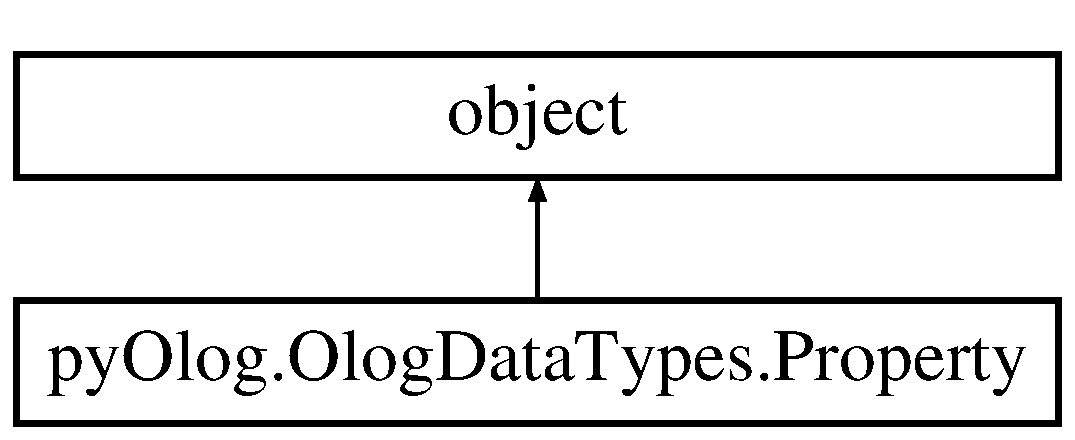
\includegraphics[height=2.000000cm]{classpyOlog_1_1OlogDataTypes_1_1Property}
\end{center}
\end{figure}
\subsection*{Public Member Functions}
\begin{DoxyCompactItemize}
\item 
def \hyperlink{classpyOlog_1_1OlogDataTypes_1_1Property_a659f1dd08e809934e762600d2f9222de}{\-\_\-\-\_\-init\-\_\-\-\_\-}
\item 
\hypertarget{classpyOlog_1_1OlogDataTypes_1_1Property_ae703878c6b7142a9d941b160e1447993}{def {\bfseries get\-Name}}\label{classpyOlog_1_1OlogDataTypes_1_1Property_ae703878c6b7142a9d941b160e1447993}

\item 
\hypertarget{classpyOlog_1_1OlogDataTypes_1_1Property_a127a50c407a76622106daa9c2ac120b1}{def {\bfseries get\-Attributes}}\label{classpyOlog_1_1OlogDataTypes_1_1Property_a127a50c407a76622106daa9c2ac120b1}

\item 
\hypertarget{classpyOlog_1_1OlogDataTypes_1_1Property_abeaa8733314ec7fd77cc8d503afaf7e0}{def {\bfseries get\-Attribute\-Names}}\label{classpyOlog_1_1OlogDataTypes_1_1Property_abeaa8733314ec7fd77cc8d503afaf7e0}

\item 
\hypertarget{classpyOlog_1_1OlogDataTypes_1_1Property_a56dbf8e69d31a92949ead2589412e82d}{def {\bfseries get\-Attribute\-Value}}\label{classpyOlog_1_1OlogDataTypes_1_1Property_a56dbf8e69d31a92949ead2589412e82d}

\item 
\hypertarget{classpyOlog_1_1OlogDataTypes_1_1Property_a3f4abd58460132ea3766d677335c6a06}{def {\bfseries \-\_\-\-\_\-cmp\-\_\-\-\_\-}}\label{classpyOlog_1_1OlogDataTypes_1_1Property_a3f4abd58460132ea3766d677335c6a06}

\end{DoxyCompactItemize}
\subsection*{Public Attributes}
\begin{DoxyCompactItemize}
\item 
\hypertarget{classpyOlog_1_1OlogDataTypes_1_1Property_a4a3026135a69326653ee052b57e45c73}{{\bfseries Attributes}}\label{classpyOlog_1_1OlogDataTypes_1_1Property_a4a3026135a69326653ee052b57e45c73}

\end{DoxyCompactItemize}


\subsection{Detailed Description}
\begin{DoxyVerb}A property consists of a unique name and a set of attributes consisting of key value pairs   
\end{DoxyVerb}
 

\subsection{Constructor \& Destructor Documentation}
\hypertarget{classpyOlog_1_1OlogDataTypes_1_1Property_a659f1dd08e809934e762600d2f9222de}{\index{py\-Olog\-::\-Olog\-Data\-Types\-::\-Property@{py\-Olog\-::\-Olog\-Data\-Types\-::\-Property}!\-\_\-\-\_\-init\-\_\-\-\_\-@{\-\_\-\-\_\-init\-\_\-\-\_\-}}
\index{\-\_\-\-\_\-init\-\_\-\-\_\-@{\-\_\-\-\_\-init\-\_\-\-\_\-}!pyOlog::OlogDataTypes::Property@{py\-Olog\-::\-Olog\-Data\-Types\-::\-Property}}
\subsubsection[{\-\_\-\-\_\-init\-\_\-\-\_\-}]{\setlength{\rightskip}{0pt plus 5cm}def py\-Olog.\-Olog\-Data\-Types.\-Property.\-\_\-\-\_\-init\-\_\-\-\_\- (
\begin{DoxyParamCaption}
\item[{}]{self, }
\item[{}]{name, }
\item[{}]{attributes = {\ttfamily None}}
\end{DoxyParamCaption}
)}}\label{classpyOlog_1_1OlogDataTypes_1_1Property_a659f1dd08e809934e762600d2f9222de}
\begin{DoxyVerb}Create a property with a unique name and attributes
>> Property('Ticket', attributes={'Id':'1234','URL':'http://trac.nsls2.bnl.gov/trac/1234'}
>> Property('Scan', attributes={'Number':'run-1234', 'script':'scan_20130117.py'}
\end{DoxyVerb}
 

The documentation for this class was generated from the following file\-:\begin{DoxyCompactItemize}
\item 
py\-Olog/Olog\-Data\-Types.\-py\end{DoxyCompactItemize}

\hypertarget{classpyOlog_1_1OlogClient_1_1PropertyDecoder}{\section{py\-Olog.\-Olog\-Client.\-Property\-Decoder Class Reference}
\label{classpyOlog_1_1OlogClient_1_1PropertyDecoder}\index{py\-Olog.\-Olog\-Client.\-Property\-Decoder@{py\-Olog.\-Olog\-Client.\-Property\-Decoder}}
}
Inheritance diagram for py\-Olog.\-Olog\-Client.\-Property\-Decoder\-:\begin{figure}[H]
\begin{center}
\leavevmode
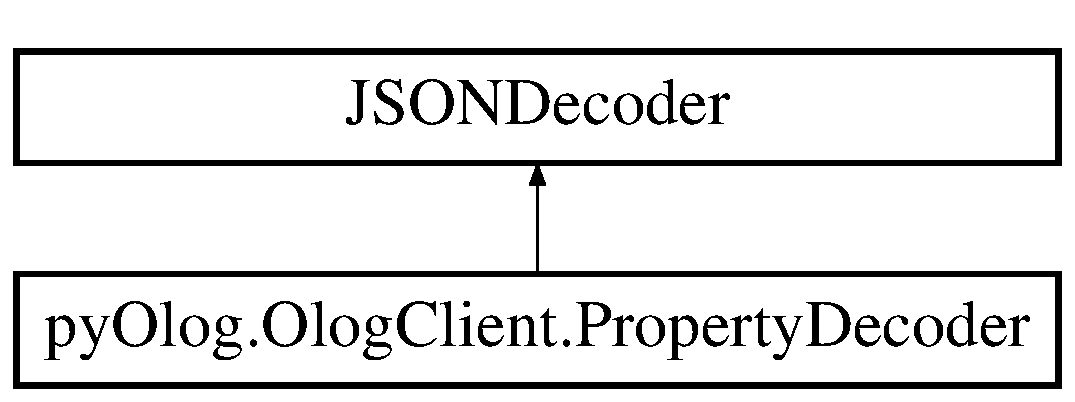
\includegraphics[height=2.000000cm]{classpyOlog_1_1OlogClient_1_1PropertyDecoder}
\end{center}
\end{figure}
\subsection*{Public Member Functions}
\begin{DoxyCompactItemize}
\item 
\hypertarget{classpyOlog_1_1OlogClient_1_1PropertyDecoder_a02e76c4a9b7e9fecf6f8b9a68a0ee379}{def {\bfseries \-\_\-\-\_\-init\-\_\-\-\_\-}}\label{classpyOlog_1_1OlogClient_1_1PropertyDecoder_a02e76c4a9b7e9fecf6f8b9a68a0ee379}

\item 
\hypertarget{classpyOlog_1_1OlogClient_1_1PropertyDecoder_ab3803ba06262664e3c55d48421be68c8}{def {\bfseries dict\-To\-Property}}\label{classpyOlog_1_1OlogClient_1_1PropertyDecoder_ab3803ba06262664e3c55d48421be68c8}

\end{DoxyCompactItemize}


The documentation for this class was generated from the following file\-:\begin{DoxyCompactItemize}
\item 
py\-Olog/Olog\-Client.\-py\end{DoxyCompactItemize}

\hypertarget{classpyOlog_1_1OlogClient_1_1PropertyEncoder}{\section{py\-Olog.\-Olog\-Client.\-Property\-Encoder Class Reference}
\label{classpyOlog_1_1OlogClient_1_1PropertyEncoder}\index{py\-Olog.\-Olog\-Client.\-Property\-Encoder@{py\-Olog.\-Olog\-Client.\-Property\-Encoder}}
}
Inheritance diagram for py\-Olog.\-Olog\-Client.\-Property\-Encoder\-:\begin{figure}[H]
\begin{center}
\leavevmode
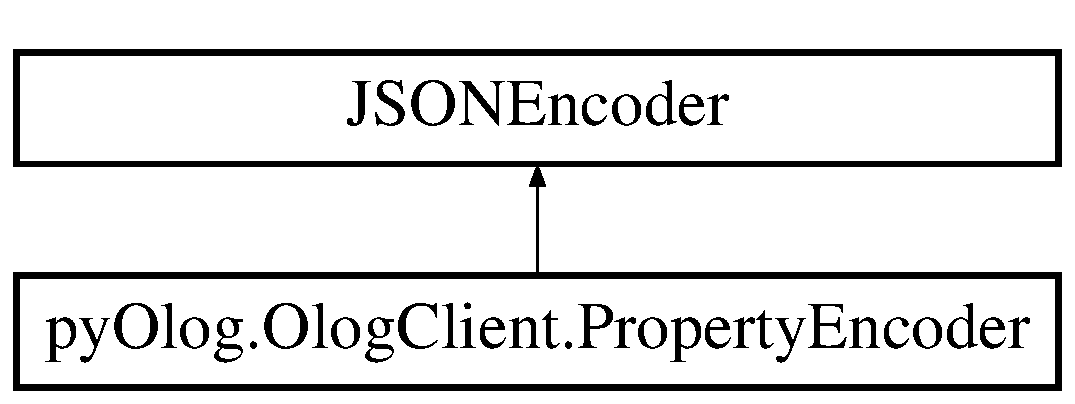
\includegraphics[height=2.000000cm]{classpyOlog_1_1OlogClient_1_1PropertyEncoder}
\end{center}
\end{figure}
\subsection*{Public Member Functions}
\begin{DoxyCompactItemize}
\item 
\hypertarget{classpyOlog_1_1OlogClient_1_1PropertyEncoder_a1c61f64455f7a5a9338f63a7174e66a5}{def {\bfseries default}}\label{classpyOlog_1_1OlogClient_1_1PropertyEncoder_a1c61f64455f7a5a9338f63a7174e66a5}

\end{DoxyCompactItemize}


The documentation for this class was generated from the following file\-:\begin{DoxyCompactItemize}
\item 
py\-Olog/Olog\-Client.\-py\end{DoxyCompactItemize}

\hypertarget{classpyOlog_1_1OlogDataTypes_1_1Tag}{\section{py\-Olog.\-Olog\-Data\-Types.\-Tag Class Reference}
\label{classpyOlog_1_1OlogDataTypes_1_1Tag}\index{py\-Olog.\-Olog\-Data\-Types.\-Tag@{py\-Olog.\-Olog\-Data\-Types.\-Tag}}
}
Inheritance diagram for py\-Olog.\-Olog\-Data\-Types.\-Tag\-:\begin{figure}[H]
\begin{center}
\leavevmode
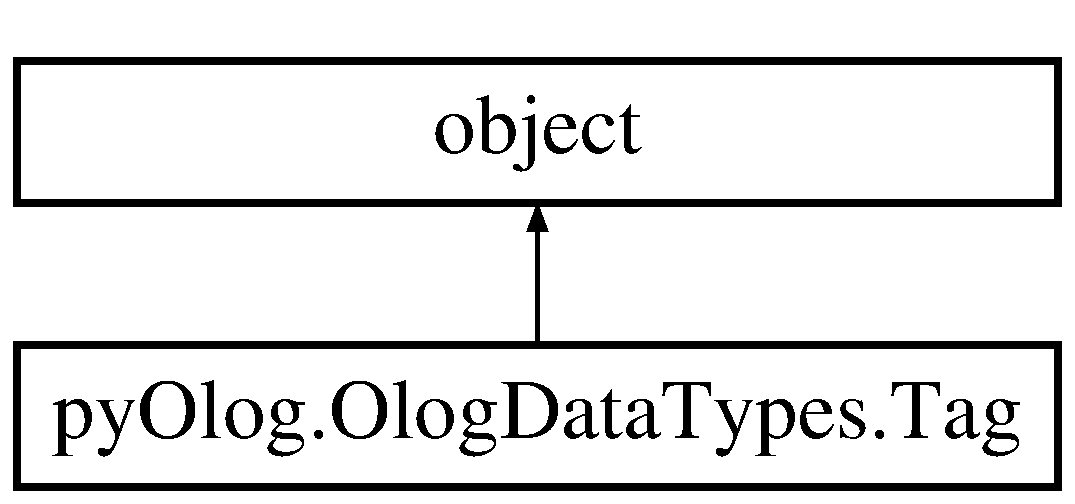
\includegraphics[height=2.000000cm]{classpyOlog_1_1OlogDataTypes_1_1Tag}
\end{center}
\end{figure}
\subsection*{Public Member Functions}
\begin{DoxyCompactItemize}
\item 
def \hyperlink{classpyOlog_1_1OlogDataTypes_1_1Tag_add599a45f6036ce7b6e14068c8ab07dd}{\-\_\-\-\_\-init\-\_\-\-\_\-}
\item 
\hypertarget{classpyOlog_1_1OlogDataTypes_1_1Tag_a568b1629e04fdf3d992e6820e0ed6c71}{def {\bfseries get\-Name}}\label{classpyOlog_1_1OlogDataTypes_1_1Tag_a568b1629e04fdf3d992e6820e0ed6c71}

\item 
\hypertarget{classpyOlog_1_1OlogDataTypes_1_1Tag_a71aa91e396e5614ce9237cf8166d4d31}{def {\bfseries get\-State}}\label{classpyOlog_1_1OlogDataTypes_1_1Tag_a71aa91e396e5614ce9237cf8166d4d31}

\item 
\hypertarget{classpyOlog_1_1OlogDataTypes_1_1Tag_a63bd5eadbe61824f9a0b152d911f4e9d}{def {\bfseries \-\_\-\-\_\-cmp\-\_\-\-\_\-}}\label{classpyOlog_1_1OlogDataTypes_1_1Tag_a63bd5eadbe61824f9a0b152d911f4e9d}

\end{DoxyCompactItemize}


\subsection{Detailed Description}
\begin{DoxyVerb}A Tag consists of a unique name, it is used to tag logEntries to enable querying and organizing log Entries
\end{DoxyVerb}
 

\subsection{Constructor \& Destructor Documentation}
\hypertarget{classpyOlog_1_1OlogDataTypes_1_1Tag_add599a45f6036ce7b6e14068c8ab07dd}{\index{py\-Olog\-::\-Olog\-Data\-Types\-::\-Tag@{py\-Olog\-::\-Olog\-Data\-Types\-::\-Tag}!\-\_\-\-\_\-init\-\_\-\-\_\-@{\-\_\-\-\_\-init\-\_\-\-\_\-}}
\index{\-\_\-\-\_\-init\-\_\-\-\_\-@{\-\_\-\-\_\-init\-\_\-\-\_\-}!pyOlog::OlogDataTypes::Tag@{py\-Olog\-::\-Olog\-Data\-Types\-::\-Tag}}
\subsubsection[{\-\_\-\-\_\-init\-\_\-\-\_\-}]{\setlength{\rightskip}{0pt plus 5cm}def py\-Olog.\-Olog\-Data\-Types.\-Tag.\-\_\-\-\_\-init\-\_\-\-\_\- (
\begin{DoxyParamCaption}
\item[{}]{self, }
\item[{}]{name, }
\item[{}]{state = {\ttfamily \char`\"{}Active\char`\"{}}}
\end{DoxyParamCaption}
)}}\label{classpyOlog_1_1OlogDataTypes_1_1Tag_add599a45f6036ce7b6e14068c8ab07dd}
\begin{DoxyVerb}Create a Tag object
>> Tag('TimingSystem')
\end{DoxyVerb}
 

The documentation for this class was generated from the following file\-:\begin{DoxyCompactItemize}
\item 
py\-Olog/Olog\-Data\-Types.\-py\end{DoxyCompactItemize}

\hypertarget{classpyOlog_1_1OlogClient_1_1TagDecoder}{\section{py\-Olog.\-Olog\-Client.\-Tag\-Decoder Class Reference}
\label{classpyOlog_1_1OlogClient_1_1TagDecoder}\index{py\-Olog.\-Olog\-Client.\-Tag\-Decoder@{py\-Olog.\-Olog\-Client.\-Tag\-Decoder}}
}
Inheritance diagram for py\-Olog.\-Olog\-Client.\-Tag\-Decoder\-:\begin{figure}[H]
\begin{center}
\leavevmode
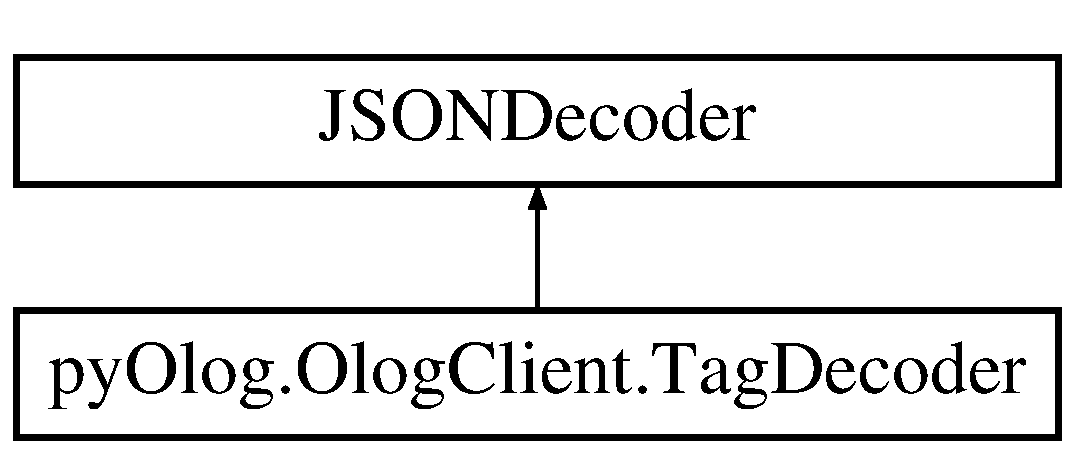
\includegraphics[height=2.000000cm]{classpyOlog_1_1OlogClient_1_1TagDecoder}
\end{center}
\end{figure}
\subsection*{Public Member Functions}
\begin{DoxyCompactItemize}
\item 
\hypertarget{classpyOlog_1_1OlogClient_1_1TagDecoder_a96a2f645cc53821489f000ffae923a24}{def {\bfseries \-\_\-\-\_\-init\-\_\-\-\_\-}}\label{classpyOlog_1_1OlogClient_1_1TagDecoder_a96a2f645cc53821489f000ffae923a24}

\item 
\hypertarget{classpyOlog_1_1OlogClient_1_1TagDecoder_a10d2ae673bfe6fef522d94257179af33}{def {\bfseries dict\-To\-Tag}}\label{classpyOlog_1_1OlogClient_1_1TagDecoder_a10d2ae673bfe6fef522d94257179af33}

\end{DoxyCompactItemize}


The documentation for this class was generated from the following file\-:\begin{DoxyCompactItemize}
\item 
py\-Olog/Olog\-Client.\-py\end{DoxyCompactItemize}

\hypertarget{classpyOlog_1_1OlogClient_1_1TagEncoder}{\section{py\-Olog.\-Olog\-Client.\-Tag\-Encoder Class Reference}
\label{classpyOlog_1_1OlogClient_1_1TagEncoder}\index{py\-Olog.\-Olog\-Client.\-Tag\-Encoder@{py\-Olog.\-Olog\-Client.\-Tag\-Encoder}}
}
Inheritance diagram for py\-Olog.\-Olog\-Client.\-Tag\-Encoder\-:\begin{figure}[H]
\begin{center}
\leavevmode
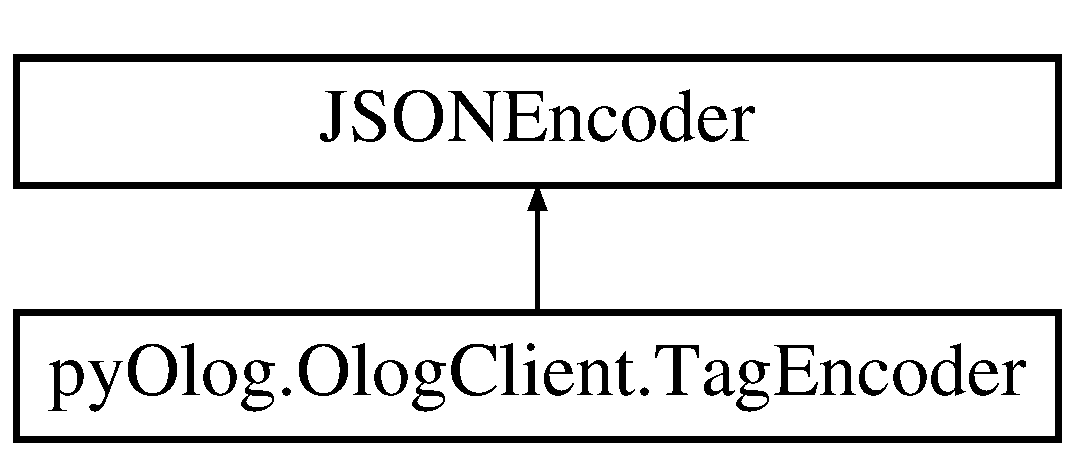
\includegraphics[height=2.000000cm]{classpyOlog_1_1OlogClient_1_1TagEncoder}
\end{center}
\end{figure}
\subsection*{Public Member Functions}
\begin{DoxyCompactItemize}
\item 
\hypertarget{classpyOlog_1_1OlogClient_1_1TagEncoder_a281c9c5b9da05bc6301a7ad8efe63d30}{def {\bfseries default}}\label{classpyOlog_1_1OlogClient_1_1TagEncoder_a281c9c5b9da05bc6301a7ad8efe63d30}

\end{DoxyCompactItemize}


The documentation for this class was generated from the following file\-:\begin{DoxyCompactItemize}
\item 
py\-Olog/Olog\-Client.\-py\end{DoxyCompactItemize}

%--- End generated contents ---

% Index
\newpage
\phantomsection
\addcontentsline{toc}{part}{Index}
\printindex

\end{document}
